% /*
%  * ----------------------------------------------------------------------------
%  * "THE BEER-WARE LICENSE" (Revision 42):
%  * Julian Klaiber and Severin Dellsperger wrote this file. As long as you retain this notice you
%  * can do whatever you want with this stuff. If we meet some day, and you think
%  * this stuff is worth it, you can buy us a beer in return.
%  * ----------------------------------------------------------------------------
%  */

\documentclass[
a4paper,
oneside,
10pt,
fleqn,
headsepline,
toc=listofnumbered, 
bibliography=totocnumbered]{scrartcl}

% deutsche Trennmuster etc.
\usepackage[T1]{fontenc}
\usepackage[utf8]{inputenc}
\usepackage[english, ngerman]{babel} % \selectlanguage{english} if  needed
\usepackage{lmodern} % use modern latin fonts

% Custom commands
\newcommand{\GITHUB}{https://github.com/jklaiber/HSR}
\newcommand{\LICENSEURL}{https://en.wikipedia.org/wiki/Beerware}
\newcommand{\LICENSE}{
"THE BEER-WARE LICENSE" (Revision 42):
Julian Klaiber and Severin Dellsperger wrote this file. As long as you retain this notice you
can do whatever you want with this stuff. If we meet some day, and you think
this stuff is worth it, you can buy us a beer in return.
}

% Jede Überschrift 1 auf neuer Seite
\let\stdsection\section
\renewcommand\section{\clearpage\stdsection}

% Multiple Authors
\usepackage{authblk}

% Include external pdf
\usepackage{pdfpages}

% Layout / Seitenränder
\usepackage{geometry}

% Inhaltsverzeichnis
\usepackage{makeidx} 
\makeindex

\usepackage{url}
\usepackage[pdfborder={0 0 0}]{hyperref}
\usepackage[all]{hypcap}
\usepackage{hyperxmp} % for license metadata

% Glossar und Abkürzungsverzeichnis
\usepackage[acronym,toc,nopostdot]{glossaries}
\setglossarystyle{altlist}
\usepackage{xparse}
\DeclareDocumentCommand{\newdualentry}{ O{} O{} m m m m } {
	\newglossaryentry{gls-#3}{
		name={#4 : #5},
		text={#5\glsadd{#3}},
		description={#6},
		#1
	}
	\makeglossaries
	\newacronym[see={[Siehe:]{gls-#3}},#2]{#3}{#4}{#5\glsadd{gls-#3}}
}
\makeglossaries

% Mathematik
\usepackage{amsmath}
\usepackage{amssymb}
\usepackage{amsfonts}
\usepackage{enumitem}

% Images
\usepackage{graphicx}
\graphicspath{{images/}} % default paths

% Boxes
\usepackage{fancybox}

%Tables
\usepackage{tabu}
\usepackage{booktabs} % toprule, midrule, bottomrule
\usepackage{array} % for matrix tables
\usepackage{multicol} %multicol

% Header and footer
\usepackage{scrlayer-scrpage}
\setkomafont{pagehead}{\normalfont}
\setkomafont{pagefoot}{\normalfont}
\automark*{section}
\clearpairofpagestyles
\ihead{\headmark}
\ohead{\AUTHOR}
\cfoot{\pagemark}

% Pseudocode
\usepackage{algorithmic}
\usepackage[linesnumbered,ruled]{algorithm2e}

% Code Listings
\usepackage{listings}
\usepackage{color}
\usepackage{beramono}

\definecolor{bluekeywords}{rgb}{0,0,1}
\definecolor{greencomments}{rgb}{0,0.5,0}
\definecolor{redstrings}{rgb}{0.64,0.08,0.08}
\definecolor{xmlcomments}{rgb}{0.5,0.5,0.5}
\definecolor{types}{rgb}{0.17,0.57,0.68}

\lstdefinestyle{visual-studio-style}{
	language=[Sharp]C,
	columns=flexible,
	showstringspaces=false,
	basicstyle=\footnotesize\ttfamily, 
	commentstyle=\color{greencomments},
	morekeywords={partial, var, value, get, set},
	keywordstyle=\bfseries\color{bluekeywords},
	stringstyle=\color{redstrings},
	breaklines=true,
	breakatwhitespace=true,
	tabsize=4,
	numbers=left,
	numberstyle=\tiny\color{black},
	frame=lines,
	showspaces=false,
	showtabs=false,
	escapeinside={£}{£},
}

\definecolor{DarkPurple}{rgb}{0.4, 0.1, 0.4}
\definecolor{DarkCyan}{rgb}{0.0, 0.5, 0.4}
\definecolor{LightLime}{rgb}{0.3, 0.5, 0.4}
\definecolor{Blue}{rgb}{0.0, 0.0, 1.0}

\lstdefinestyle{cevelop-style}{
	language=C++,  
	columns=flexible,
	showstringspaces=false,     
	basicstyle=\footnotesize\ttfamily, 
	keywordstyle=\bfseries\color{DarkPurple},
	commentstyle=\color{LightLime},
	stringstyle=\color{Blue}, 
	escapeinside={£}{£}, % latex scope within code      
	breaklines=true,
	breakatwhitespace=true,
	showspaces=false,
	showtabs=false,
	tabsize=4,
	morekeywords={include,ifndef,define},
	numbers=left,
	numberstyle=\tiny\color{black},
	frame=lines,
}

\lstdefinestyle{eclipse-style}{
	language=Java,  
	columns=flexible,
	showstringspaces=false,     
	basicstyle=\footnotesize\ttfamily, 
	keywordstyle=\bfseries\color{DarkPurple},
	commentstyle=\color{LightLime},
	stringstyle=\color{Blue}, 
	escapeinside={£}{£}, % latex scope within code      
	breaklines=true,
	breakatwhitespace=true,
	showspaces=false,
	showtabs=false,
	tabsize=4,
	morekeywords={length},
	numbers=left,
	numberstyle=\tiny\color{black},
	frame=lines,
}
\lstset{style=eclipse-style}



% Theorems \begin{mytheo}{title}{label}
\usepackage{tcolorbox}
\tcbuselibrary{theorems}
\newtcbtheorem[number within=section]{definiton}{Definition}%
{fonttitle=\bfseries}{def}
\newtcbtheorem[number within=section]{remember}{Merke}%
{fonttitle=\bfseries}{rem}
\newtcbtheorem[number within=section]{hint}{Hinweis}%
{fonttitle=\bfseries}{hnt}

% Colors
\definecolor{strings}{HTML}{448c25}
\definecolor{comments}{HTML}{aaaaaa}
\definecolor{keywords}{HTML}{aa3d8c}
\definecolor{background}{HTML}{f4f4f4}
\definecolor{numbers}{HTML}{a884e0}

% Default style
\lstdefinestyle{default}{
    backgroundcolor=\color{background},
    basicstyle=\ttfamily\small,
    breakatwhitespace=true,
    breaklines=true,
    commentstyle=\color{comments},
    deletekeywords={},
    escapeinside={}{},
    extendedchars=true,
    frame=lines,
    keepspaces=true,
    keywordstyle=\color{keywords},
    morekeywords={},
    numbers=left,
    numberstyle=\ttfamily\color{numbers},
    rulecolor=\color{numbers},
    showspaces=false,
    showstringspaces=false,
    showtabs=false,
    stepnumber=1,
    stringstyle=\color{strings},
    tabsize=2,
}
\lstset{
    style=default,
    columns=fullflexible
}

% Language cisco-config
\lstdefinelanguage{cisco-config}{
    morekeywords={no,ip,ipv6,int,interface},
    morecomment=[l][\color{comments}]{!},
    numbers=none
}

% Language cisco-teminal
\lstdefinelanguage{cisco-terminal}{
    morecomment=[l][\color{strings}]{\#},
    morecomment=[l][\color{strings}]{>},
    numbers=none
}

\lstdefinelanguage{bash}{
    numbers=none
}

\makeatletter
\@addtoreset{section}{part}
\makeatother

% Boxes
\tcbuselibrary{most}

\usepackage{fontawesome}

% \cmd{...}
\newcommand{\cmd}[1]{\texttt{#1}}

% Info Box
\definecolor{infobar}{HTML}{02cefc}
\definecolor{infobackground}{HTML}{baf0fc}
\newcommand{\info}[2]{
    \begin{tcolorbox}[
        arc = 0mm,
        boxrule = 0pt,
        breakable,
        before skip=11pt,
        before skip=11pt,
        title = \faInfo~#1,
        fonttitle = \sffamily\bfseries,
        coltitle = white,
        colbacktitle = infobar,
        colback = infobackground,
        toptitle=2mm,
        bottomtitle=2mm,
        top=4mm,
        bottom=4mm
    ]
    #2
    \end{tcolorbox}
}

% Warning Box
\definecolor{warnbar}{HTML}{f90053}
\definecolor{warnbackground}{HTML}{fcc4d7}
\newcommand{\warn}[2]{
    \begin{tcolorbox}[
        arc = 0mm,
        boxrule = 0pt,
        breakable,
        before skip=11pt,
        before skip=11pt,
        title = \faWarning~#1,
        fonttitle = \sffamily\bfseries,
        coltitle = white,
        colbacktitle = warnbar,
        colback = warnbackground,
        toptitle=2mm,
        bottomtitle=2mm,
        top=4mm,
        bottom=4mm
    ]
    #2
    \end{tcolorbox}
}

% Login Information Box
\definecolor{loginbar}{HTML}{FA8A05}
\definecolor{loginbackground}{HTML}{F3D4AF}
\newcommand{\login}[2]{
    \begin{tcolorbox}[
        arc = 0mm,
        boxrule = 0pt,
        breakable,
        before skip=11pt,
        before skip=11pt,
        title = \faKey~#1,
        fonttitle = \sffamily\bfseries,
        coltitle = white,
        colbacktitle = loginbar,
        colback = loginbackground,
        toptitle=2mm,
        bottomtitle=2mm,
        top=4mm,
        bottom=4mm
    ]
    #2
    \end{tcolorbox}
}

\definecolor{settingborder}{HTML}{0066CC}
\definecolor{settingcontent}{HTML}{E5F2FA}
\newcommand{\setting}[1]{
    \begin{tcolorbox}[
        colback = settingcontent,
        colframe = settingborder
    ]
    You can find the settings under: \\
    \textbf{\clicks{~#1}}
    \end{tcolorbox}
}

\definecolor{configurationborder}{HTML}{005700}
\definecolor{configurationcontent}{HTML}{e6ffcc}
\newcommand{\configuration}[2]{
    \begin{tcolorbox}[
        colback = configurationcontent,
        colframe = configurationborder
    ]
    \textbf{Configuration:}\\
    To reach an output like below you only have to add/change the following parameters 
    ~#1
    You can find the settings under: \\
    \textbf{\clicks{~#2}}
    \end{tcolorbox}
}


\usepackage{multirow}

% URLs
\urlstyle{rm}
\definecolor{link}{HTML}{0450f2}
\hypersetup{
    colorlinks,
    allcolors=.,
    urlcolor=link,
}

% \url[display]{url} or \url{url}
\renewcommand{\url}[2][]{%
    \ifstrempty{#1}{%
        \burlalt{#2}{#2}%
    }{%
        \burlalt{#1}{#2}%
    }%
}

% Clicks
\newcommand{\clicks}[1]{%
    $\foreach \n [count=\ni] in {#1}{%
        \ifnum\ni=1%
            \textit{\n}%
        \else%
            \rightarrow \textit{\n}%
        \fi%
    }$%
}

% Keystrokes
\newcommand{\keys}[1]{%
    $\foreach \n [count=\ni] in {#1}{%
        \ifnum\ni=1%
            \textit{\n}%
        \else%
            + \textit{\n}%
        \fi%
    }$%
}

% Dokumentinformationen
\newcommand{\SUBJECT}{Zusammenfassung}
\newcommand{\TITLE}{Informations und Codierungstheorie}

\loadglsentries{glossar}

% pdf metadata
\hypersetup{
	pdfauthor={\AUTHOR},
	pdftitle={\SUBJECT \TITLE},
	pdfcopyright={\LICENSE},
	pdflicenseurl={\LICENSEURL}
}

\begin{document}
	
\begin{titlepage}

\newcommand{\HRule}{\rule{\linewidth}{0.5mm}} % Defines a new command for the horizontal lines, change thickness here

\center % Center everything on the page
 
%----------------------------------------------------------------------------------------
%	HEADING SECTIONS
%----------------------------------------------------------------------------------------

\textsc{\LARGE \INSTITUTE}\\[1.5cm] % Name of your university/college
\textsc{\Large \SUBJECT}\\[0.5cm] % Major heading such as course name

%----------------------------------------------------------------------------------------
%	TITLE SECTION
%----------------------------------------------------------------------------------------

\HRule \\[0.6cm]
{ \huge \bfseries \TITLE}\\[0.4cm] % Title of your document
\HRule \\[1.5cm]

%----------------------------------------------------------------------------------------
%	AUTHOR SECTION
%----------------------------------------------------------------------------------------

\begin{minipage}{0.4\textwidth}
\begin{flushleft} \large
\emph{Author:}\\
\AUTHORONE % Your name
\end{flushleft}
\end{minipage}
~
\begin{minipage}{0.4\textwidth}
\begin{flushright} \large
\emph{} \\
\AUTHORTWO
\end{flushright}
\end{minipage}\\[2cm]

%----------------------------------------------------------------------------------------
%	DATE SECTION
%----------------------------------------------------------------------------------------

{\large \today}\\[2cm] % Date, change the \today to a set date if you want to be precise

%----------------------------------------------------------------------------------------
%	LOGO SECTION
%----------------------------------------------------------------------------------------


\includegraphics[width=10cm,height=5cm,keepaspectratio]{ressources/hsr_logo.jpg}\\[1cm] 
 
%----------------------------------------------------------------------------------------

\vfill % Fill the rest of the page with whitespace

\end{titlepage} 	


\section{Teil Steffen}

\subsection{Umrechnungen}
\begin{figure}[h!]
	\centering
	\begin{minipage}[t]{0.5\textwidth}
		\centering
		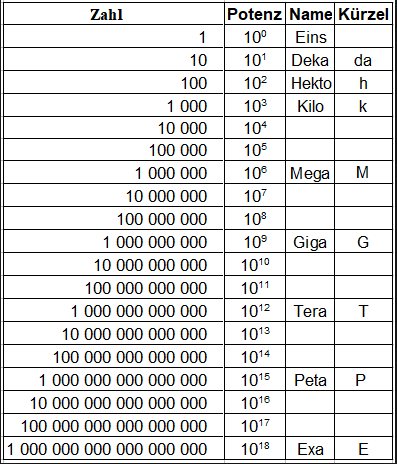
\includegraphics[width=0.9\linewidth]{images/zehnerpotenzen}
		\caption{Zehnerpotenzen Tabelle}
		\label{fig:zehnerpotenzen}
	\end{minipage}
	\begin{minipage}[t]{0.5\textwidth}
		\centering
		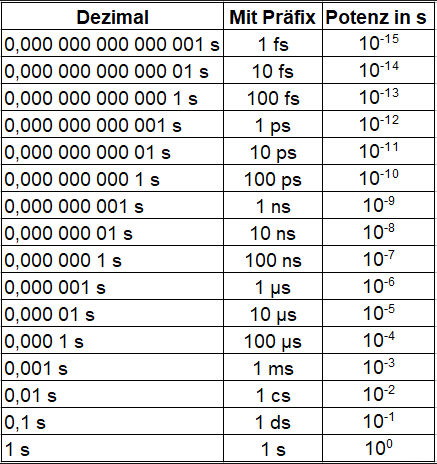
\includegraphics[width=0.9\linewidth]{images/sekundeneinheiten}
		\caption{Zeiteinheiten}
		\label{fig:zeiteinheiten}
	\end{minipage}
\end{figure}

\subsection{Signal-to-noise Ratio und Pegelplan}

\subsubsection{Thermische Rauschleistung}
\textbf{Formel:}\\
\\
$N[dBm]=-174dBm+10log_1_0(\Delta f) \\ \Delta f = Frequenzintervall[Hz]$

\textbf{Beispiel:} \\
Systembandbreite = 4GHz
$n=-174dBm+10log_{10}(4*10^9)=-78dBm$\\


\clearpage
\subsubsection{Pegelplan}
\textbf{SNR Berechnung: }Der SNR für den Pegelplan berechnet sich wie folgt \textbf{Thermische Rauschleistung + Abstand (aus der Aufgabenstellung)} \\

\textbf{Signaldynamik:} $S_m_a_x-S_m_i_n$ in dB

\begin{figure}[h!]
	\centering
	\begin{minipage}[t]{0.8\textwidth}
		\centering
		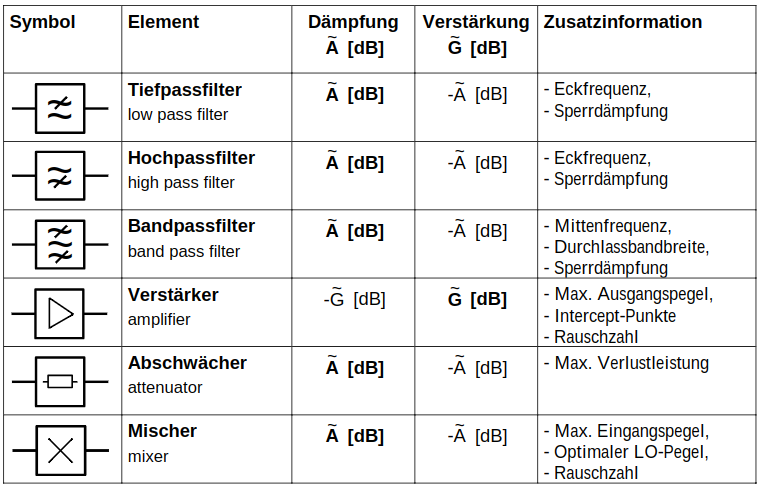
\includegraphics[width=0.9\linewidth]{images/pegelplan_elemente}
		\caption{Pegelplan Elemente}
		\label{fig:pegelplanelemente}
	\end{minipage}
	\begin{minipage}[t]{0.8\textwidth}
		\centering
		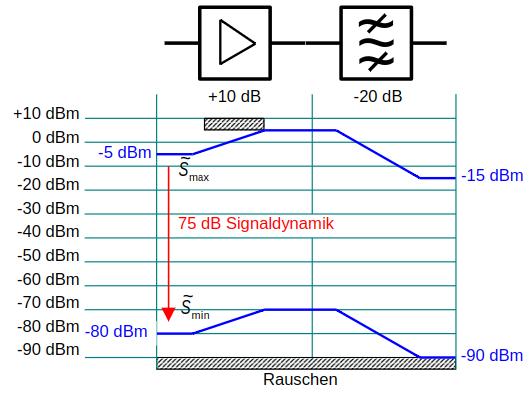
\includegraphics[width=0.9\linewidth]{images/pegelplan_beispiel}
		\caption{Beispiel Pegelplan}
		\label{fig:pegelplanbeispiel}
	\end{minipage}
\end{figure}
\clearpage

\subsection{Abtastung von Signalen}
\textbf{Aliasing} tritt auf, wenn im abzutastenden Signal Frequenzanteile vorkommen, die höher sind als die halbe Abtastfrequenz. Signal > $1/2*Abtastfrequenz$. Durch vorschalten eines Tiefpassfilters mit einer Grenzfrequenz $f_g<f_s/2$, kann Aliasing vermieden werden.
\\
\textbf{Frage:} Was bewirkt die gezielte Wahl der Smapling Frequenz $f_s=f_0$?
\textbf{Antwort:} Das Sampling mit der Trägerfrequenz $f_0$ bewirkt eine Verschiebung des Datensignals in das Basisband und damit eine Produktdemodulation mit $f_0$.

\subsection{Dauer und Bandbreite von Einzelpulsen}
\subsubsection{Vorgehen Amplitudendichte}
\textbf{Fragestellung:} Wie kann S(0), d.h. die Amplitudendichte bei der Frequenz f=0 Hz, einfach aus dem Verlauf des Pulses berechnet werden? Geben Sie die Formel für S(0), sowie den numerischen Wert in [V/Hz] an.\\
\\
\textbf{Lösung:} $S(0)=\int_{-\infty }^{\infty}s(t)dt=\int_{-T}^{T}s(t)dt=AT$ \\
\\
d.h. die Gesamtfläche unter der Dreiecksfunktion s(t).\\
\\
\textbf{Hinweis:} \\
Bei Recktecksignalen wäre es $2*AT$\\
Bei ms führt es zu mV/Hz

\subsubsection{Energie berechnen}
$E=\int_{-\infty}^{\infty}\frac{s^2(t)}{R}dt=\frac{1}{R}\int_{-\infty}^{\infty}s^2(t)dt=\frac{3}{4}*\frac{A^2T}{R}$
\\ 
\\
Achtung: 3/4 und T ist modular \\
\\
\textbf{Hinweis:} Resultat wenn ms dann mWs (Beispiel: 3/4mWs = 0.75mJ)

\subsubsection{Dauer eines Pulses berechnen}
\textbf{Formel:} $E=\frac{A^2\tau}{R}=\frac{3}{4}*\frac{A^2T}{R}$ \\
\textbf{nach $\tau$ auflösen $\tau$ in ms oder s}\\
\\
Achtung: 3/4 und T ist modular

\subsubsection{Bandbreite}
\textbf{Formel:} $E=\frac{|S(0)|^2*B}{R}=\frac{A^2T^2B}{R}=\frac{3}{4}*\frac{A^2T}{R}$\\ $B=\frac{3}{4}*\frac{1}{T}$ und damit $B=\frac{3}{4}kHz=0.75kHz$\\
\\
Achtung: 3/4 und T ist modular
\clearpage

\subsubsection{Zeit-Bandbreitenprodukt}
Wie gross ist das Zeit-Bandbreitenprodukt B\tau ?\\
\\
\textbf{Formel:} $B\tau=\frac{3}{4}*\frac{1}{T}*\frac{3}{4}*T$
\\
\\
Achtung: 3/4 und T ist modular
\\
\textbf{Hinweis:} kHz und ms lösen sich auf = keine Masseinheit

\subsection{Leitungscodes}

\begin{table}[h!]
\centering
\begin{tabular}{|l|l|l|l|l|}
\hline
\multirow{2}{*}{Leitungscode} & \multicolumn{2}{l|}{DC-Freiheit} & \multicolumn{2}{l|}{Taktinformation} \\ \cline{2-5} 
                              & Ja             & Nein            & Ja               & Nein              \\ \hline
Bipolarer NRZ Code            &                & X               &                  & X                 \\ \hline
Unipolarer NRZ Code           & X               &                &                 &  X                 \\ \hline
Unipolarer NRZ Mark Code      & *              &  *               &                 &  X                 \\ \hline
Bipolarer Manchester-Code     & X              &                 & X                &                   \\ \hline
Unipolarer Manchester-Code    &               &  X               & X                &                   \\ \hline
Bipolarer AMI Code            & X              &                 &                 &  X                 \\ \hline
Unipolarer RZ Code			 &	X			  & 			   & 				&	X				\\ \hline
\end{tabular}
\caption{Nur Nullstellen}
\caption{*=Nicht entscheidbar kommt auf vorheriges Zeichen an.}
\end{table}

\begin{table}[h!]
\centering
\begin{tabular}{|l|l|l|l|l|}
\hline
\multirow{2}{*}{Leitungscode} & \multicolumn{2}{l|}{DC-Freiheit} & \multicolumn{2}{l|}{Taktinformation} \\ \cline{2-5} 
                              & Ja             & Nein            & Ja               & Nein              \\ \hline
Bipolarer NRZ Code            &                & X               &                  & X                 \\ \hline
Unipolarer NRZ Code           &                & X               &                  & X                 \\ \hline
Unipolarer NRZ Mark Code      & X              &                 & X                &                   \\ \hline
Bipolarer Manchester-Code     & X              &                 & X                &                   \\ \hline
Unipolarer Manchester-Code    & X              &                 & X                &                   \\ \hline
Bipolarer AMI Code            & X              &                 & X                &                   \\ \hline
Unipolarer RZ Code			 &				  & X		       & X				&					\\ \hline
\end{tabular}
\caption{Nur Einsstellen}
\end{table}

\clearpage
\subsection{Modulationsarten}
\subsubsection{Beispiel}
\begin{figure}[h!]
	\centering
	\begin{minipage}[t]{0.9\textwidth}
		\centering
		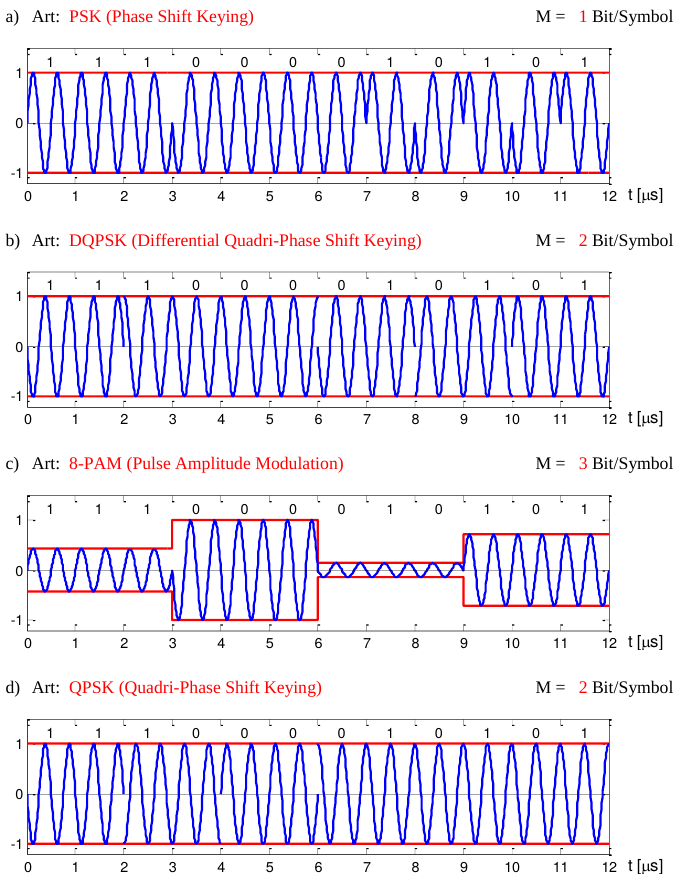
\includegraphics[width=0.9\linewidth]{images/modulationsarten}
		\caption{Modulationsarten Beispiel}
		\label{fig:modulationsartenbeispiel}
	\end{minipage}
\end{figure}
\clearpage

\subsection{Tonhöhenverschiebung von Audiosignalen}
\subsubsection{Mickey Mouse}
\textbf{Lösung 1:} 
\begin{itemize}
	\item Elimination des oberen Seitenbandes (USB) durch ein Tiefpassfilter mit der Grendfrequenz (diese auslesen was muss wohin geschoben werden)
	\item Demodulation mit einer LO-Frequenz von X (Auslesen), welches das untere Seitenband (LSB) mit einem Frequenzshift von X in das Basisband zurückschiebt
\end{itemize}
\textbf{Lösung 2:}
\begin{itemize}
	\item Elimination des unteren Seitenbandes (LSB) durch ein Hochpassfilter mit der Grenzfrequenz X (auslesen)
	\item Demodulation mit einer LO-Frequenz von X (auslesen), welches das obere Seitenband (USB) mit einem Frequenzshift von X in das Basisband zurückschiebt.
\end{itemize}
\textbf{Massnahmen nach der Verschiebung:} 
\begin{itemize}
	\item Durch die Demodulation ensteht eine Spektrumskomponente bei der doppelten Trägerfrequenz von ca. 16kHz
	\item Die hörbaren Frequenzanteile können mit einem Tiefpassfilter eliminiert werden.
\end{itemize}

\section{Teil Meili}

\subsection{Entscheidungsgehalt}
Mass für den Aufwand der zur Bildung einer Nachricht bzw. für die Entscheidung einer Nachricht notwendig ist.
\\
\\
$H_0=log_2(N)[bit]$

\subsection{Entscheidungsfluss}
$H_0^*=\frac{log_2(N)}{\tau}[\frac{bit}{s}]$ \\
\\
wobei $\tau$ die Zeit zur Übertragung eines Quellzeichens.

\subsection{Ergebnis und Ergebnismenge}
\textbf{Definition:} Die Menge aller möglichen Ausgänge eines Zufallsvorgangs heisst \textbf{Ergebnismenge} und wird mit $\omega$ bezeichnet. Ein einzelnes Element heisst Ergebnis. Wir notieren die Anzahl aller Elemente von $\omega$ d.h. die Anzahl aller Ergebnisse mit $| \omega |$

\subsection{Informationsgehalt}
\textbf{Definition:} Der Informationsgehalt eines Zeichens sagt aus, wie viele Elementarentscheidungen zur Bestimmung dieses Zeichens zu treffen sind.\\
\\
$I(x_{k})=log_2(\frac{1}{p(x_k)})[bit]$
\\
\\
\textbf{Taschenrechner:} icth\textbackslash i\_info(x)
\subsection{Entropie}
\textbf{Definition:} Die Entropie bezeichnet den mittleren Informationsgehalt der Quelle. Sie zeigt also auf, wie viele Elementarentscheidungen die Quelle/Senke im Mittel pro Zeichen treffen muss. \\
\\
$H(X)=\sum_{k=1}^{N}p(x_k)*I(x_k)=\sum_{k=1}^{N}p(x_k)*log_2(\frac{1}{p(x_k)})[bit/Zeichen]$
\\ \\
Durchschnittliche Anzahl Entscheidungen die von der Quelle getrofen werden müssen. \\ \\
\textbf{Taschenrechner:} icth\textbackslash h\_entropie({Wahrscheinlichkeiten})

\subsection{Redundanz}
Der mittlere Informationsgehalt, die Entropie, einer Quelle/Senke wird maximal wenn beide Zeichen gleich oft vorkommen. \\ \\
Je kleiner die Entropie desto grösser die Redundanz. Wenn alle Zeichen gleich wahrscheinlich sind ist die Entropie maximal und die Redundanz = 0. \\ \\
$R_Q=H_0-H(X)[bit/Zeichen]$

\subsection{Kanalmodell}
\begin{figure}[h!]
	\centering
	\begin{minipage}[t]{0.9\textwidth}
		\centering
		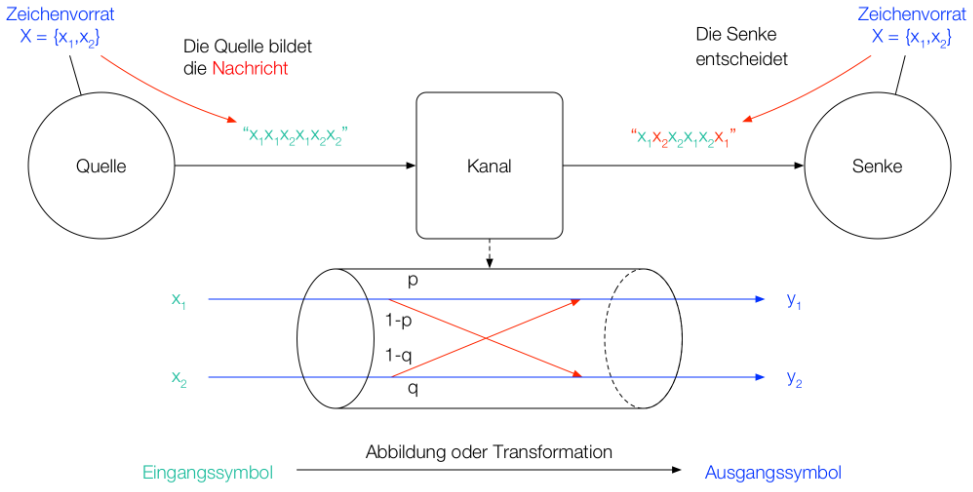
\includegraphics[width=0.9\linewidth]{images/kanalmodell}
		\caption{Kanalmodell}
		\label{fig:kanalmodell}
	\end{minipage}
\end{figure}
\clearpage

\subsubsection{Kanalmatrix}
\begin{figure}[h!]
	\centering
	\begin{minipage}[t]{0.9\textwidth}
		\centering
		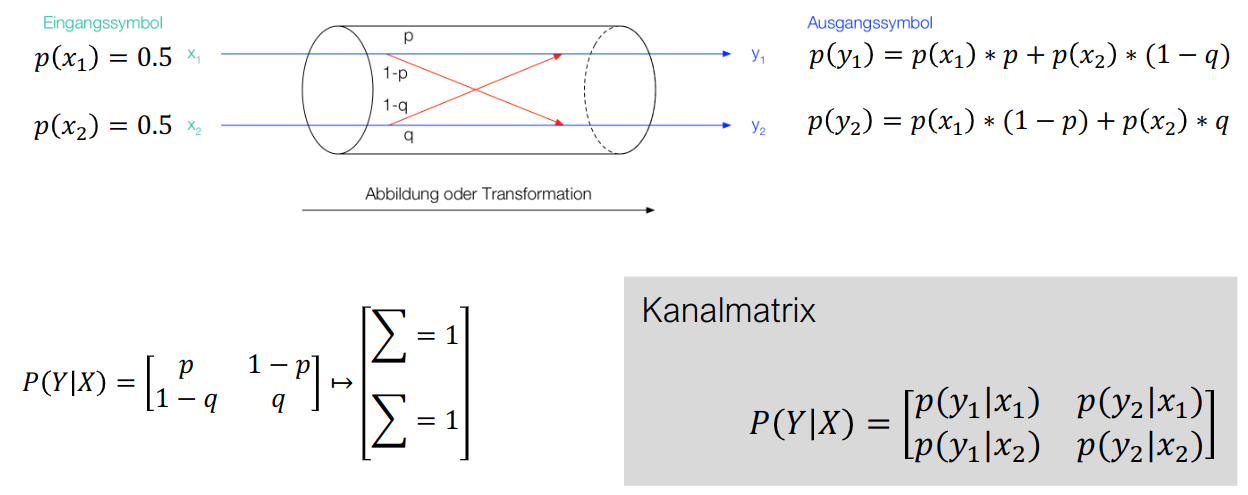
\includegraphics[width=0.9\linewidth]{images/kanalmatrix}
		\caption{Kanalmatrix}
		\label{fig:kanalmatrix}
	\end{minipage}
	\begin{minipage}[t]{0.9\textwidth}
		\centering
		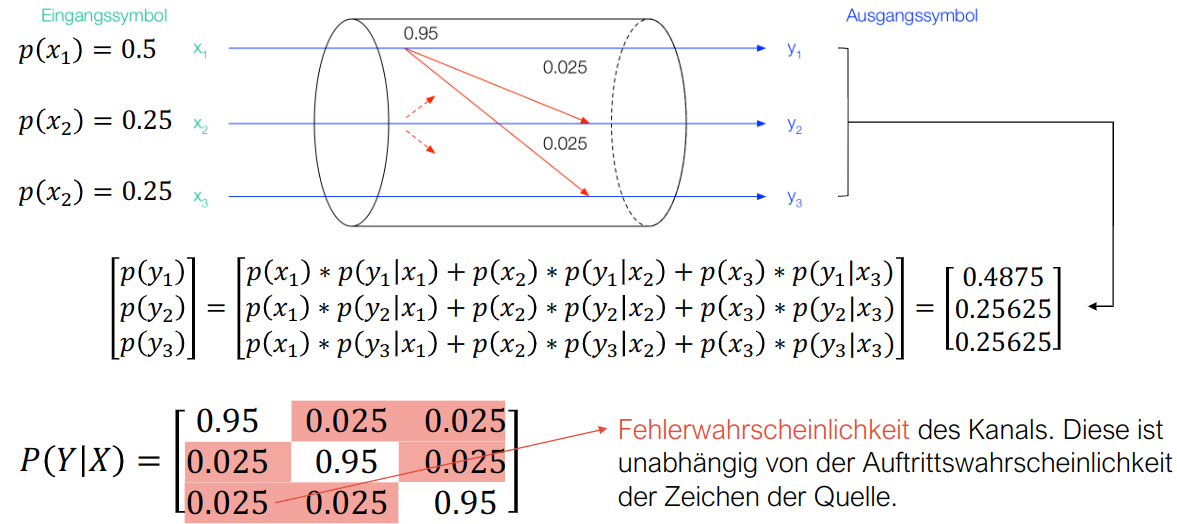
\includegraphics[width=0.9\linewidth]{images/beispielkanalmatrix}
		\caption{Kanalmatrix Beispiel}
		\label{fig:kanalmatrixbeispiel}
	\end{minipage}
\end{figure}
\textbf{Frage:} Wie kann die Kanalmatrix eines Kanals praktisch ermittelt werden?\\
\textbf{Lösung:} Viele Messungen durchführen und aus diesen die Häufigkeiten berrechnen. Daraus kann dann die Kanalmatrix erstellt werden.
\clearpage

\subsubsection{Maximum-Likelihood Verfahren}
\begin{minipage}[t]{0.9\textwidth}
	\centering
	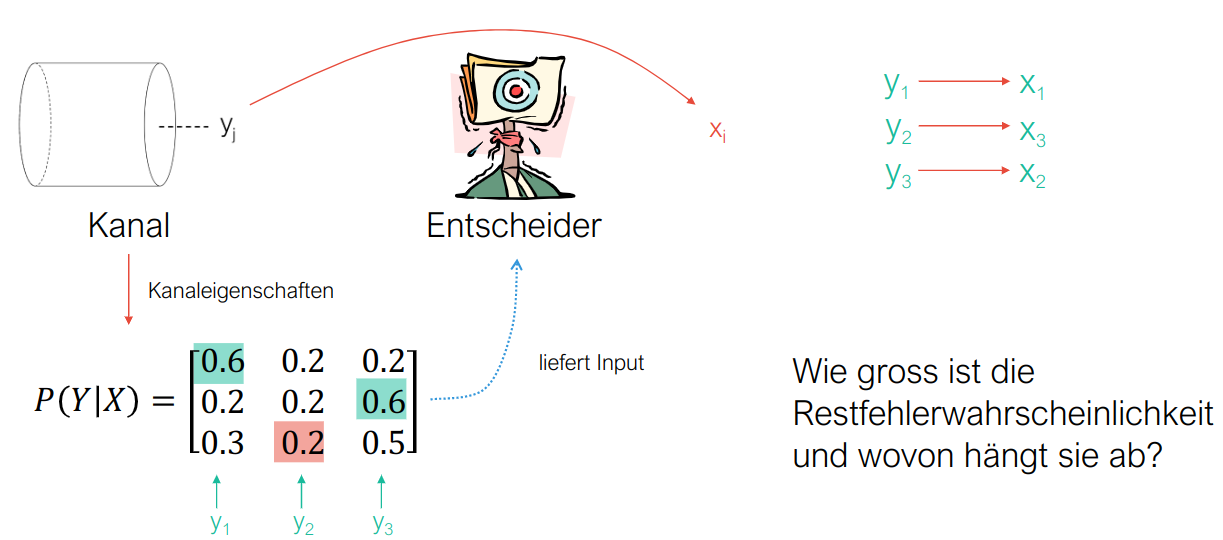
\includegraphics[width=0.9\linewidth]{images/maximumlikelihood}
	\caption{Maximum-Likelihood Verfahren}
	\label{fig:maximumlikelihood}
\end{minipage}
\\
\\
\textbf{Restfehlerwahrscheinlichkeit:} \\ \\
$p(keineFehler)=0.6*p(x_1)+0.2*p(x_3)+0.6*p(x_2)$ \\
$p(Restfehlerwahrscheinlichkeit)=1-p(keineFehler)$
\\
\\
\textbf{Taschenrechner:} icth\textbackslash res\_ err\_ prop

\clearpage
\subsubsection{Transinformation}
\begin{minipage}[t]{0.9\textwidth}
	\centering
	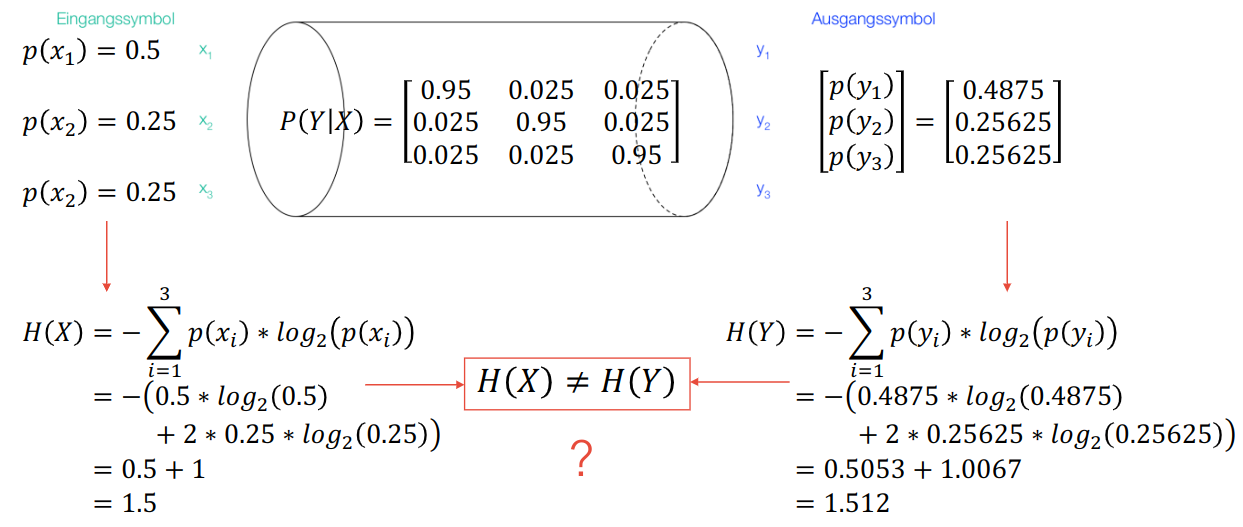
\includegraphics[width=0.9\linewidth]{images/transinformation}
	\caption{Transinformation}
	\label{fig:transinformation}
\end{minipage}
\\
\\
\begin{minipage}[t]{0.9\textwidth}
	\centering
	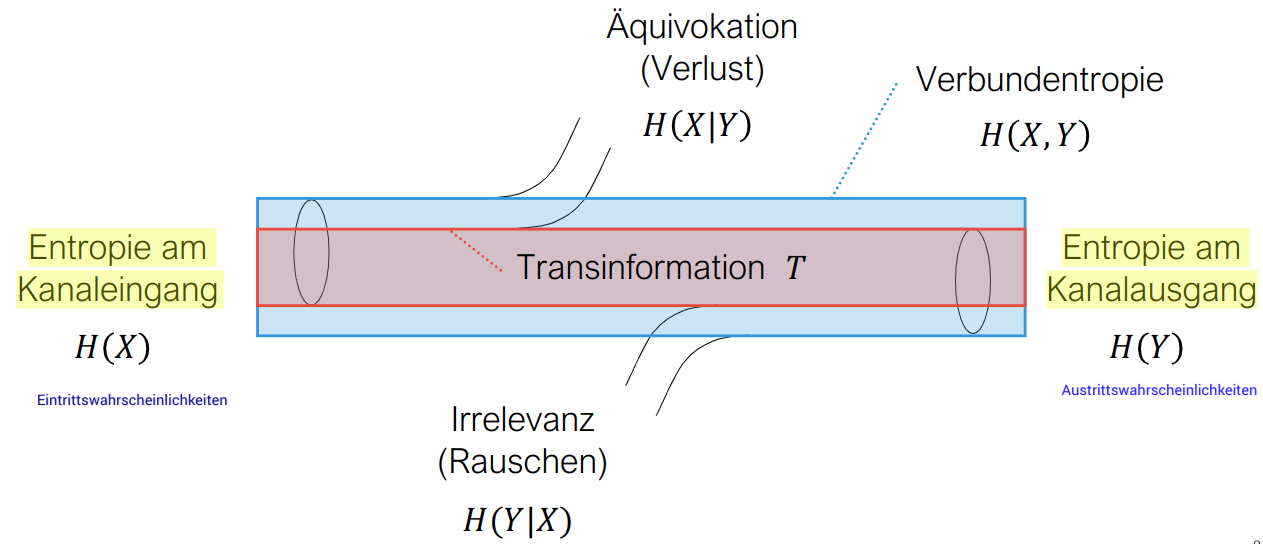
\includegraphics[width=0.9\linewidth]{images/transinformationkanal}
	\caption{Transinformation am Kanal}
	\label{fig:transinformationkanal}
\end{minipage}
\subsubsection{Transinformation Berechnung}
$T=H(X)-H(X|Y)[bit/Zeichen]$ \\
\\
$T=H(Y)-H(Y|X)[bit/Zeichen]$

\subsubsection{Äquivokation (Verlust)}
$H(X|Y)=-\sum_j^n\sum_j^np(x_j,y_j)*log_2(p(x_j|y_j))$
\\
\\
\begin{itemize}
	\item Auch Rückschlussentropie genannt
	\item Ungewissheit über das gesendete Zeichen bei bekanntem Empfangszeichen
	\item Merke: Ist der Kanal fehlerfrei, so ist die Äquivokation gleich 0
\end{itemize}

\subsubsection{Irrelevanz (Rauschen)}
$H(X|Y)=-\sum_j^n\sum_j^np(x_j,y_j)*log_2(p(y_j|x_j))$
\\
\\
\begin{itemize}
	\item Auch Streuentropie genannt
	\item Ungewissheit der empfangenen Zeichen bei vorgegeben Sendezeichen
\end{itemize}
\\
\\
\textbf{Taschenrechner:} icth\textbackslash float h\_ yx

\subsubsection{Verbundentropie}
$H(X|Y)=-\sum_j^n\sum_j^np(x_j,y_j)*log_2(p(x_j,y_j))$
\\
\\
Der mittlere Informationsgehalt über alle Zeichen (bestehend aus einem Zeichen der Quelle und einem Zeichen der Senke) \\
\\
$p(x, y) = p(x) * p(y | x)$

\subsubsection{Bedingte Entropie}
$H(Y|X)=H(X,Y)-H(X)$

\subsubsection{Symbolrate Rmax}
$T*Bandbreite$
\clearpage

\subsection{Blockcodes}
\subsubsection{Nachrichtenzahl}
$m=2^k-k-1$

\subsubsection{Hamming Distanz}
\textbf{Hammingdistanz h=} Kürzeste Distanz (Änderungen) von einem gültigen Codewort zum nächsten gültigen Codewort.
\begin{figure}[h!]
	\centering
	\begin{minipage}[t]{0.6\textwidth}
		\centering
		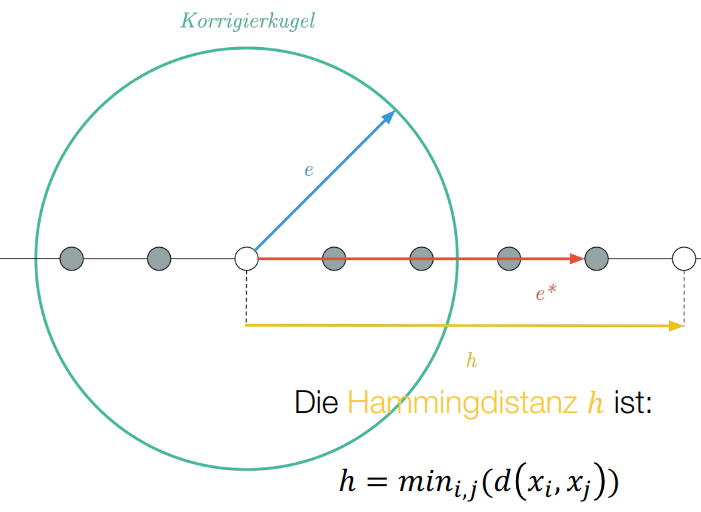
\includegraphics[width=0.9\linewidth]{images/hammingdistanz}
		\caption{Hammingdistanz}
		\label{fig:hammingdistanz}
	\end{minipage}
\end{figure}

\subsubsection{Kontrollstellen für Codewort ermitteln}
\begin{itemize}
	\item Codewort über Matrix schreiben
	\item Kontrollieren ob 1 und 1 matched (markieren)
	\item Auf jeder Zeile alle matched 1 zusammenzählen mod 2 rechnen
\end{itemize}
\begin{figure}[h!]
	\centering
	\begin{minipage}[t]{0.6\textwidth}
		\centering
		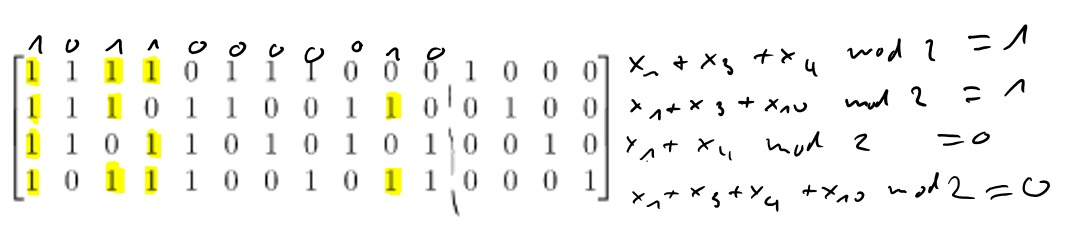
\includegraphics[width=0.9\linewidth]{images/codewort}
		\caption{Codewort ermitteln Beispiel}
		\label{fig:codewortermitteln}
	\end{minipage}
\end{figure}
\clearpage

\subsection{Hamming Codeblock aus Messwerten}
\begin{figure}[h!]
	\centering
	\begin{minipage}[t]{0.9\textwidth}
		\centering
		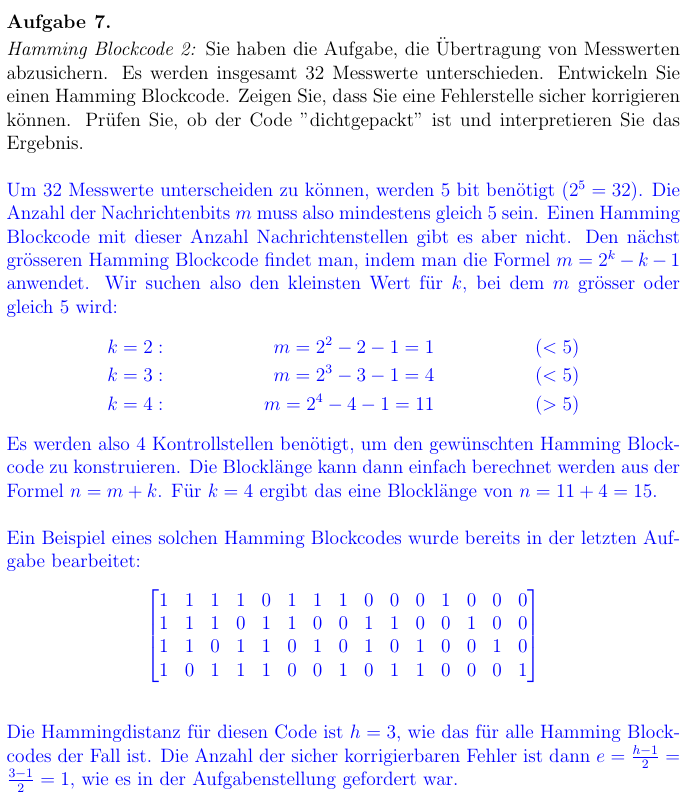
\includegraphics[width=0.9\linewidth]{images/aufgabe7}
		\caption{Hammming Codeblock Beispiel}
		\label{fig:aufgabe7}
	\end{minipage}
\end{figure}
\clearpage

\subsubsection{Fehlersyndrom ermitteln}
Wenn $x_1$ falsch dann aus Matrix Spalte 1 herausschreiben. \\
Wenn zwei Fehler beide Spalten addieren.

\subsubsection{Anzahl der sicher erkennbaren Fehler}
$e^*=h-1$

\subsubsection{Anzahl der sicher korrigierbaren Fehler}
\textbf{h gerade:} \\
\\
$h=2e+2=>e=\frac{h-2}{2}$
\\
\\
\textbf{h ungerade:} \\
\\
$h=2e+1=>e=\frac{h-1}{2}$ \\
\\
Wenn mehr als die Anzahl der sicher korrigierbaren Fehler auftreten, dann wird entweder falsch korrigiert oder der Fehler wird nicht gefunden.

\subsubsection{Anzahl berechnen}
\textbf{Anzahl möglicher Codeworte:} $2^{m+k}$
\\
\textbf{Anzahl gültiger Codeworte:} $2^m$
\\


\subsubsection{Dichtgepackt}
Der Coderaum ist dichtgepackt, wenn sich alle Codewörter(gültige und ungültige) in einer Korrigierkugel befinden. Es sei:
\begin{itemize}
	\item \textbf{n} die Dimension des Codes (Anzahl aller CW=$2^n$)
	\item \textbf{m} die Dimension der Nachrichten (Anzahl aller gültigen CW=$2^m$)
	\item \textbf{k} die Dimension der Kontrollstellen mit $n=m+k$
\end{itemize} 

\textbf{Wichtig:} Falls Hammingdistanz gerade --> kann nicht dichtgepackt sein. \\
\\
$2^m*\sum_{w=0}^e\binom{n}{w}\leqslant2^n$

\subsubsection{Blockcodes}
\begin{figure}[h!]
	\centering
	\begin{minipage}[t]{0.6\textwidth}
		\centering
		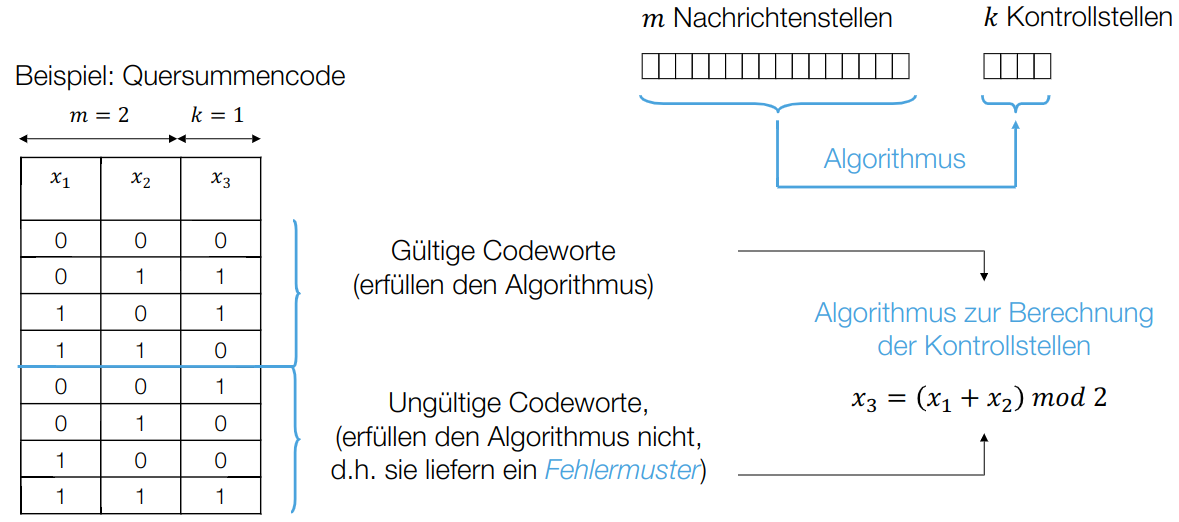
\includegraphics[width=0.9\linewidth]{images/blockcodes}
		\caption{Blockcodes}
		\label{fig:blockcodes}
	\end{minipage}
\end{figure}

\subsubsection{Hamming Code}
\begin{itemize}
	\item Hammingdistanz immer 3
	\item Linearer Blockcode
\end{itemize}

\subsection{Zyklische Codes}
\begin{itemize}
	\item Generatormatrix (Prüfmatrix) kann durch Generatorpolynom beschrieben werden.
	\item Höchster Grad des Generatorpolynoms entspricht der Anzahl Kontrollstellen (gilt auch für CRC)
	\item $n=2^k-1$
	\item $n=m+k$
\end{itemize}

\subsubsection{Kontrollstellen bestimmen}
\textbf{Mehrfachaddition:} \\
\\
\begin{figure}[h!]
	\centering
	\begin{minipage}[t]{0.4\textwidth}
		\centering
		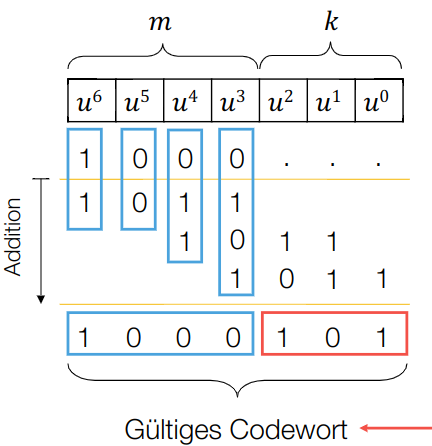
\includegraphics[width=0.9\linewidth]{images/mehrfachaddition}
		\caption{Mehrfachaddition}
		\label{fig:mehrfachaddition}
	\end{minipage}
\end{figure}

\textbf{Polynomdivision:}\\
\\
\begin{figure}[h!]
	\centering
	\begin{minipage}[t]{0.6\textwidth}
		\centering
		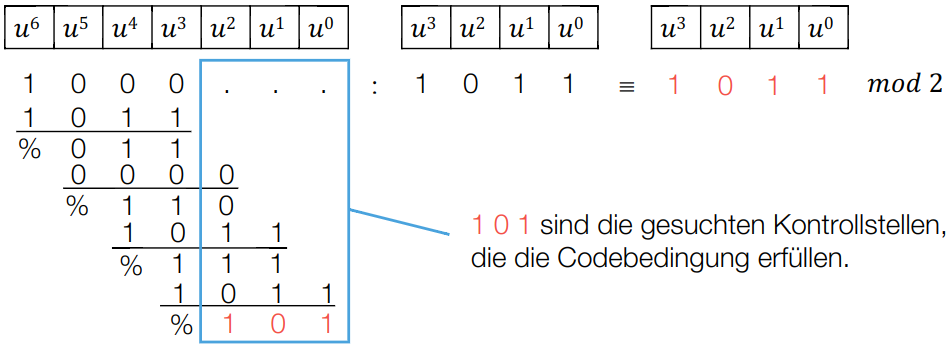
\includegraphics[width=0.9\linewidth]{images/polynomdivision}
		\caption{Polynomdivision}
		\label{fig:polynomdivision}
	\end{minipage}
\end{figure}

Das Generatorpolynom von \textbf{1011} lautet => $1*u^3+0*u^2+1*u^1+1*u^0$

\subsubsection{Prüfen der Codebedingung}
\begin{figure}[h!]
	\centering
	\begin{minipage}[t]{0.6\textwidth}
		\centering
		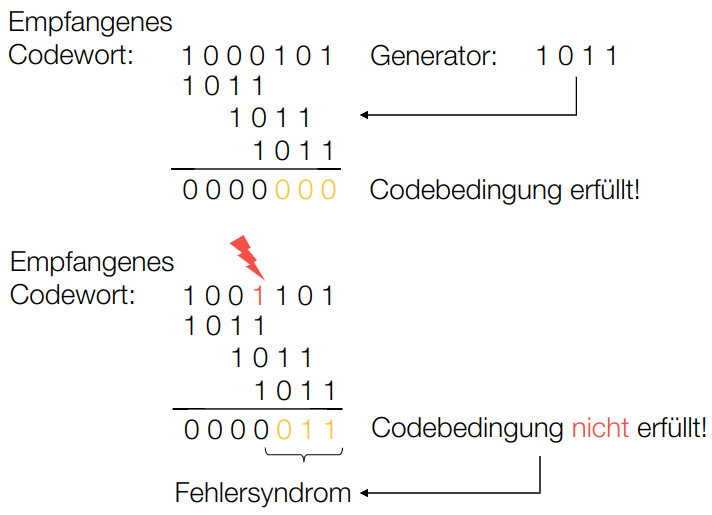
\includegraphics[width=0.9\linewidth]{images/wortpruefen}
		\caption{Beispiel}
		\label{fig:wortpruefen}
	\end{minipage}
\end{figure}

\subsubsection{Prüfmatrix}
\begin{figure}[h!]
	\centering
	\begin{minipage}[t]{0.9\textwidth}
		\centering
		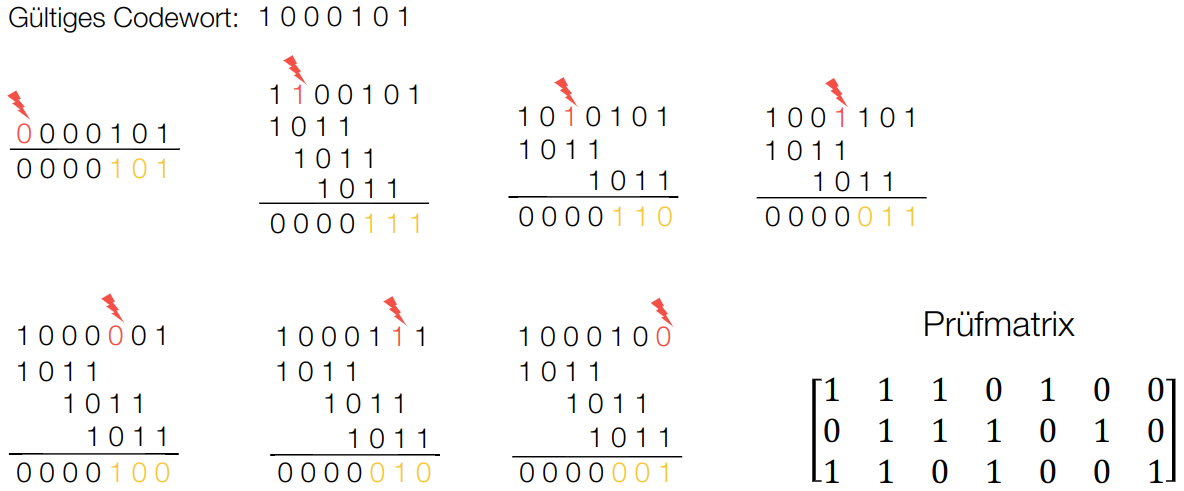
\includegraphics[width=0.9\linewidth]{images/pruefmatrix}
		\caption{Prüfmatrix}
		\label{fig:pruefmatrix}
	\end{minipage}
\end{figure}

\subsubsection{CRC Code}
\begin{itemize}
	\item Hammingdistanz h = 4
	\item Wird gebildet durch die Multiplikation eines primitiven Polynoms mit dem Term (1+x)
\end{itemize}
$g(x)=(p(x)*(1+x))mod2$ \\
\\
\textbf{Abramson-Code:} $2^{k-1}-1$

\subsubsection{Rückgekoppeltes Schieberegister}
Schieberegister von $1+x^2+x^4+x^5$
\begin{figure}[h!]
	\centering
	\begin{minipage}[t]{0.7\textwidth}
		\centering
		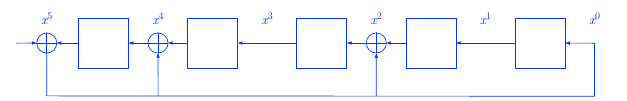
\includegraphics[width=0.9\linewidth]{images/schieberegister}
		\caption{Schieberegister}
		\label{fig:schieberegister}
	\end{minipage}
\end{figure}
\clearpage

\subsection{Faltungscodes}
\textbf{Bedeutung:} \\
\begin{itemize}
	\item (3,1,2) Faltungscode
		\subitem 3 Ausgänge
		\subitem 1 Eingang
		\subitem 2 Speicherzellen
\end{itemize}

\begin{figure}[h!]
	\centering
	\begin{minipage}[t]{0.7\textwidth}
		\centering
		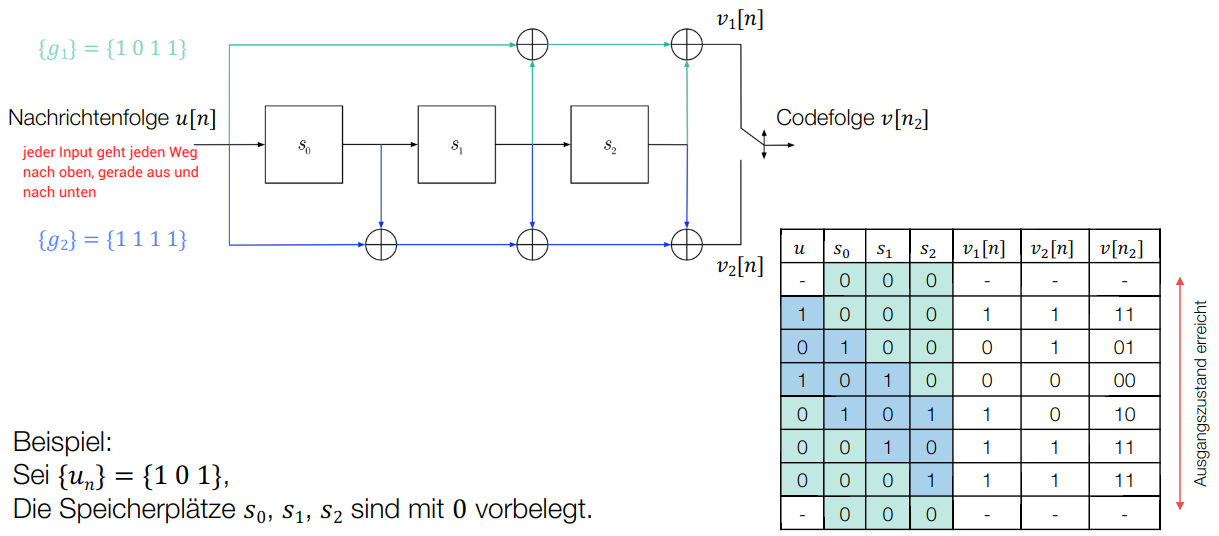
\includegraphics[width=0.9\linewidth]{images/encoderschaltung}
		\caption{Encoderschaltung}
		\label{fig:encoderschaltung}
	\end{minipage}
	\begin{minipage}[t]{0.6\textwidth}
		\centering
		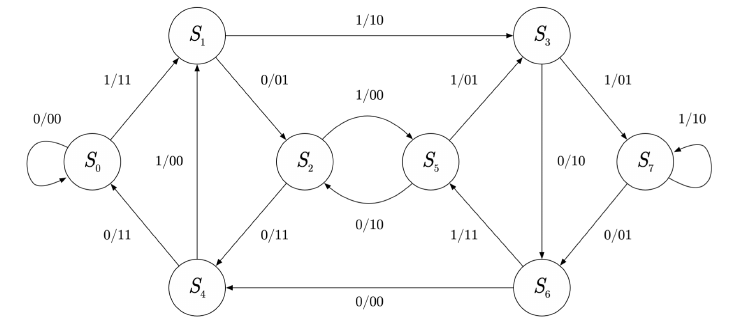
\includegraphics[width=0.9\linewidth]{images/zustandsdarstellung}
		\caption{Zustandsdarstellung}
		\label{fig:zustandsdarstellung}
	\end{minipage}
		\begin{minipage}[t]{0.5\textwidth}
		\centering
		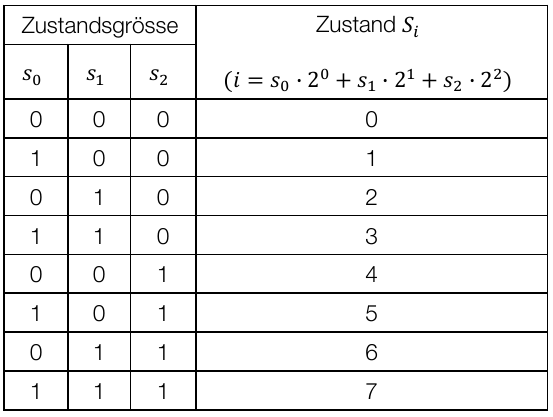
\includegraphics[width=0.9\linewidth]{images/zustandstabelle}
		\caption{Zustandstabelle}
		\label{fig:zustandstabelle}
	\end{minipage}
\end{figure}

\subsubsection{Encodergedächtnis und Tailbits}
\textbf{Encodergedächtnis:} Anzahl Speicherstellen \\
\textbf{Tailbits:} Anzahl Speicherstellen\\

\subsubsection{Blockcoderate}
Blockcoderate R = $\frac{AnzahlCodierteBits}{AnzahlGeneratorpolynom*(AnzahlCodierteBits+AnzahlSpeicherstellen}$

\subsubsection{Guter Code?}
Es handelt sich um einen guten Code wenn der Unterschied der Ausgabe bei einem Zustandsübergang immer maximal ist.

\subsubsection{Katastrophaler Code?}
Wenn es Zyklen ohne Gewichtszunahme gibt dann ist es ein katastrophaler Code.

\subsubsection{Anzahl Bits für Berechnung der Ausgangsbits}
Immer das aktuelle Bit + Anzahl Speicherstellen.

\subsubsection{Impulsantwort der Encoderschaltung}
\begin{figure}[h!]
	\centering
	\begin{minipage}[t]{0.7\textwidth}
		\centering
		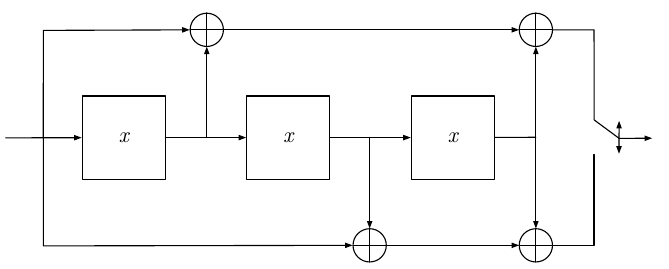
\includegraphics[width=0.9\linewidth]{images/impulsantwortbeispiel}
		\caption{Impulsantwort Beispiel}
		\label{fig:impulsantwortbeispiel}
	\end{minipage}
\end{figure}

\textbf{Anzahl Bits:} Aktuelles + 3 Speicherstellen = 4 \\
\\
\textbf{Impulsantwort:} \\
$u[n]=1,0,0,0$ \\
$v[n]=11,01,10,11$ \\
\\
\textbf{Als Polynom dargestellt:} \\
$g_1(x)=1+x+^3$ \\
$g_2(x)=1+x^2+x^3$

\subsubsection{Anzahl Zustände}
$2^{AnzahlSpeicherstellen}$\\
\clearpage

\subsection{Quellencodierung}
\subsubsection{Mittlere Codewortlänge}
$L=\sum_{i=1}^Np(x_i)*L(x_i)[bit/Zeichen]$ \\
\\
\begin{itemize}
	\item Die diskreten Zeichen der Quelle werden auf binäre CW abgebildet
	\item Günstig ist wenn die mittlere Codewortlänge L möglichst klein ist
\end{itemize}

\subsubsection{Shannon'sches Codierungstheorem}
\begin{itemize}
	\item Für jede beliebige zugehörige Binärcodierung mit Präfixeigenschaft ist die mittlere Codewortlänge nicht kleiner als die Entropie \textbf{H(X)}
	\item Für jede beliebige Quelle kann eine Binärcodierung gefunden werden, so dass die folgende Ungleichung gilt:
		\subitem $H(X)\leqslant L\leqslant  H(X)+1$
\end{itemize}
\textbf{Redundanz der Quelle:} \\
$R_Q=H_0-H(X)[bit/Zeichen]$ \\
\\
\textbf{Redundanz des Codes:} \\
$R_C=L-H(X)[bit/Zeichen]$ \\
\begin{figure}[h!]
	\centering
	\begin{minipage}[t]{0.7\textwidth}
		\centering
		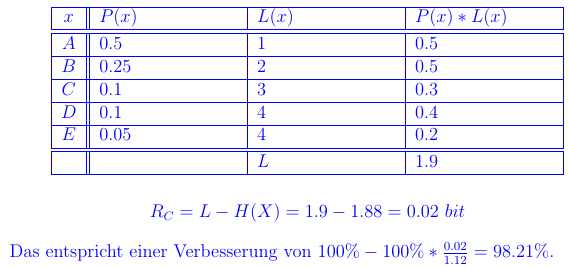
\includegraphics[width=0.9\linewidth]{images/redundanzdescodes}
		\caption{Redundanz des Codes berechnen}
		\label{fig:redundanzdescodes}
	\end{minipage}
\end{figure}
\clearpage

\begin{figure}[h!]
	\centering
	\begin{minipage}[t]{0.9\textwidth}
		\centering
		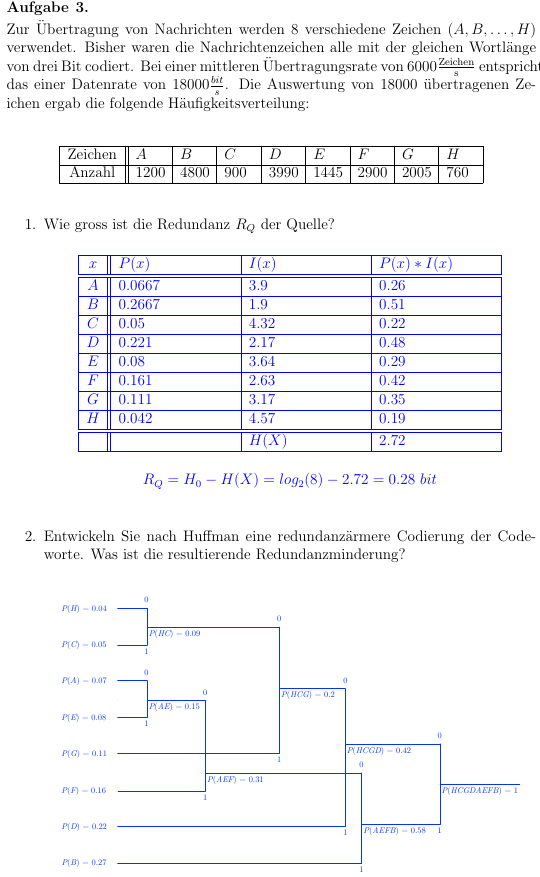
\includegraphics[width=0.9\linewidth]{images/beispielhuffmann1}
		\caption{Huffmann Beispiel 1}
		\label{fig:huffmannbeispiel1}
	\end{minipage}
\end{figure}
\clearpage

\begin{figure}[h!]
	\centering
	\begin{minipage}[t]{0.9\textwidth}
		\centering
		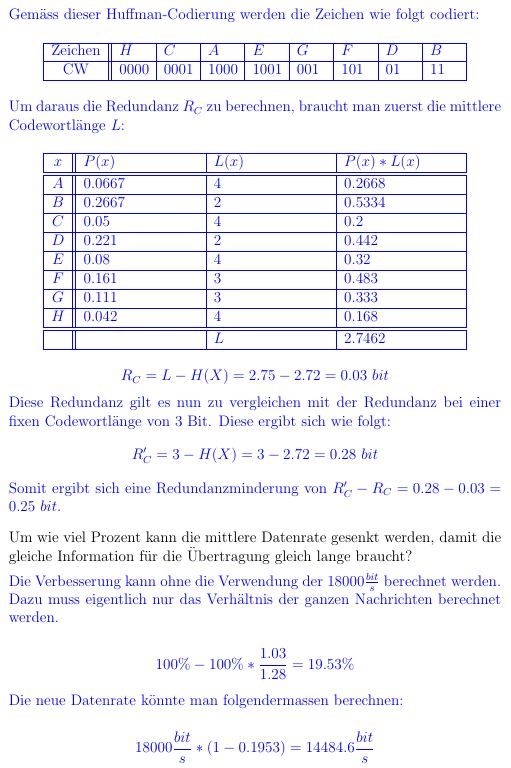
\includegraphics[width=0.9\linewidth]{images/beispielhuffmann2}
		\caption{Huffmann Beispiel 2}
		\label{fig:huffmannbeispiel2}
	\end{minipage}
\end{figure}
\clearpage

\subsubsection{Markov Diagramm}
\begin{figure}[h!]
	\centering
	\begin{minipage}[t]{0.7\textwidth}
		\centering
		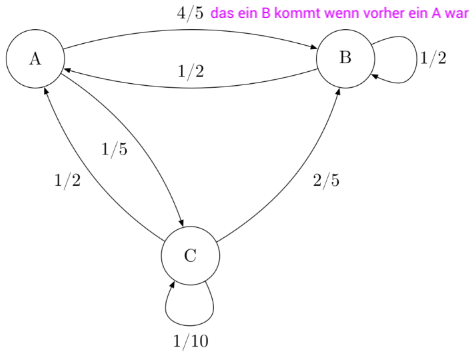
\includegraphics[width=0.9\linewidth]{images/markov}
		\caption{Markov Diagram}
		\label{fig:markov}
	\end{minipage}
\end{figure}


\subsubsection{Diskrete Quelle mit Gedächtnis}
\begin{figure}[h!]
	\centering
	\begin{minipage}[t]{0.9\textwidth}
		\centering
		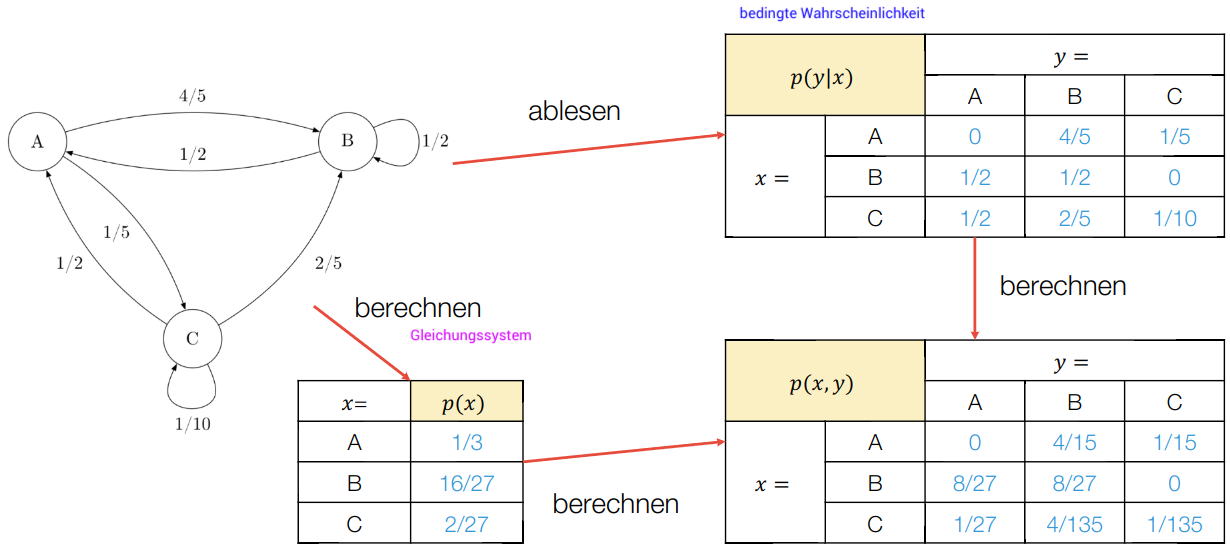
\includegraphics[width=0.9\linewidth]{images/diskretequellemitgedaechtnis}
		\caption{Beispiel}
		\label{fig:diskretequelle}
	\end{minipage}
\end{figure}
\clearpage

\textbf{Taschenrechner Gleichungssystem:}\\
\begin{figure}[h!]
	\centering
	\begin{minipage}[t]{0.5\textwidth}
		\centering
		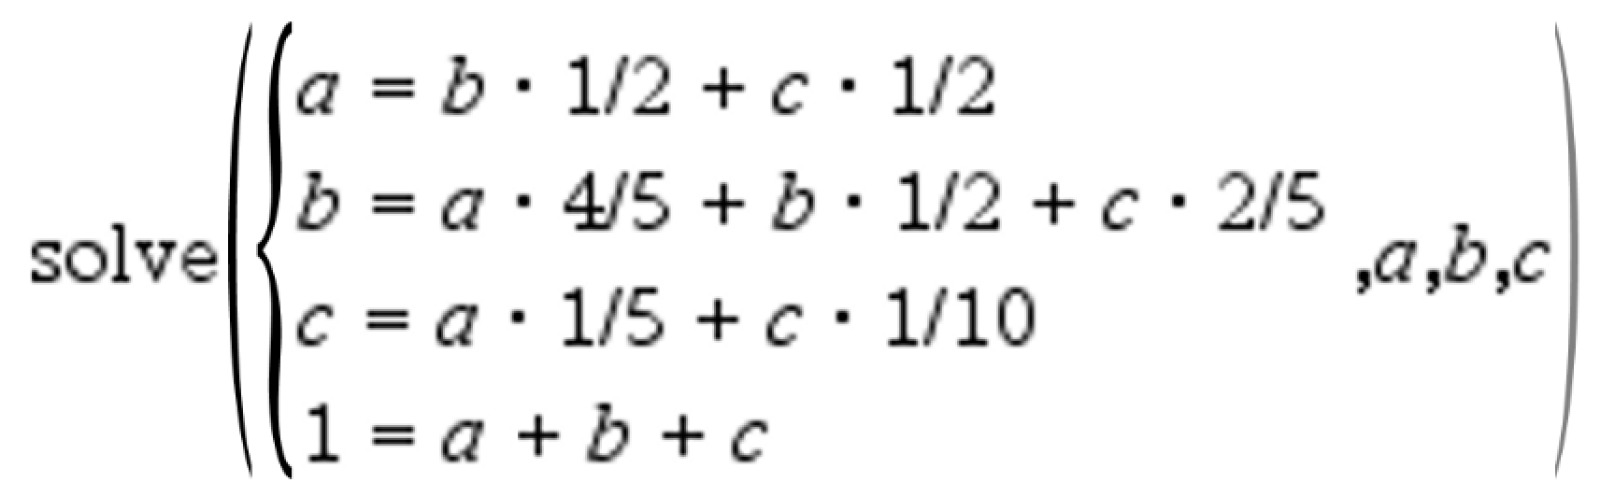
\includegraphics[width=0.9\linewidth]{images/gls}
		\caption{Gleichungssystem Nspire}
		\label{fig:gls}
	\end{minipage}
\end{figure}

\subsection{Komprimierung}
Das Ziel der Datenkomprimierung ist, den Aufwand der Datenspeicherung und Datenübertragung zu reduzieren.\\
\\
D.h. Entfernen von Redundanz und Irrelevanz 
\begin{figure}[h!]
	\centering
	\begin{minipage}[t]{0.7\textwidth}
		\centering
		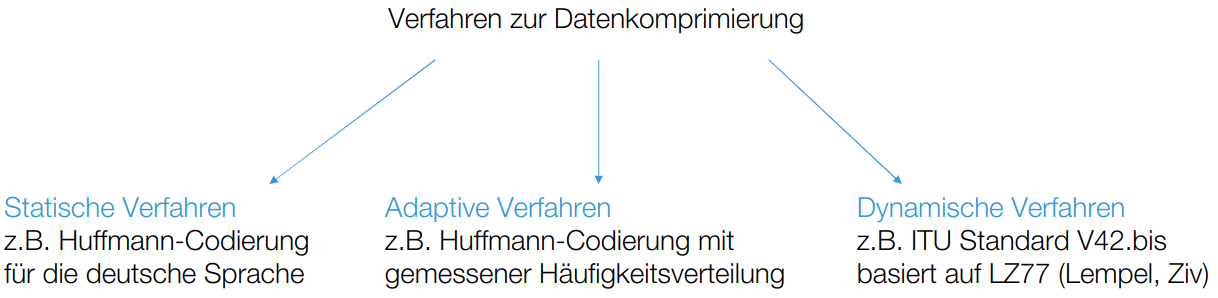
\includegraphics[width=0.9\linewidth]{images/datenkomprimierung}
		\caption{Komprimierungsarten}
		\label{fig:komprimierung}
	\end{minipage}
\end{figure}

\subsubsection{Huffman-Codierung}
Verfahren zur Entwicklung eines Codes mit minimaler mittlerer Codewortlänge. \\
Rekursives Verfahren, d.h. der Binärbaum wird nicht von der Wurzel, sondern von den Blättern aus entwickelt. \\
\\
\textbf{Verfahren:}
\begin{itemize}
	\item Ordne die Zeichen gemäss ihrer Auftrittswahrscheinlichkeit
	\item Die beiden Zeichen mit der kleinsten Auftrittswahrscheinlichkeit haben die gleiche CW-Länge \textbf{$L_N$}
	\item Sei \textbf{$L_N$} die mittlere CW-Länge für eine Quelle mit N Zeichen und $L_{N-1}$ die mittlere CW-Länge für den Fall, dass die beiden letzten zu einem einzigen Zeichen zusammengefasst werden.
\end{itemize}

\subsection{Kryptologie}
\begin{itemize}
	\item Symmetrische Verfahren (Ein Schlüssel für Ver/Entschlüsseln)
		\subitem Caesar Chiffre
		\subitem Transpositionverfahren
	\item Asymmetrische Verfahren (Ein Schlüssel Ver- Ein Schlüssel Entschlüsseln)
		\subitem Modulo Rechnung und inverse Zahlen
		\subitem Eulerfunktion
		\subitem Satz von Euler
		\subitem RSA
		\subitem Euklidischer Algorithmus und Inverser Euklidischer Algorithmus
		\subitem Grosse Zahlen
	\item Substitutionsverfahren
		\subitem Die Buchstaben des Klartextes werden durch andere Symbole ersetzt
	\item Transpositionsverfahren
		\subitem Die Zeichenfolge des Klartextes wird nicht ersetzt sondern verwürfelt
	\item Playfair-Chiffre
		\subitem Gruppen von Zeichen werden codiert
\end{itemize}

\subsubsection{Caesar Chiffre}
\textbf{Knacken: } \\
Bei einer Cesar-Verschlüsselung werden die Häufigkeiten der Quellzeichen nicht verwürfelt. Ist die Zielsprache bekannt ist auch das häufigste Zeichen der Sprache bekannt. Ist der Erhaltene Code gross genug kannn mit einer einfachen Häufigkeitsanalyse der Schlüssel ermittelt werden.


\subsubsection{RSA}
$n=p*q$ \\
$\phi(n)=(p-1)*(q-1)$ \\



\end{document}